% ISAS 2026 submission (double-blind). Compile on Overleaf: pdfLaTeX + BibTeX.
% Every number from the evaluation is marked "% RESULT". Main results: seeds 1-3, pooled;
% ablations: application B, seed 1. Source: artifacts/evaluation-v13 (summary.json and
% analysis/paper_numbers.py, which prints every number below).
\documentclass[conference]{IEEEtran}
\IEEEoverridecommandlockouts

\usepackage{cite}
\usepackage{amsmath,amssymb}
\usepackage{graphicx}
\usepackage{booktabs}
\usepackage{multirow}
\usepackage{xcolor}
\usepackage{tikz}
\usetikzlibrary{positioning,arrows.meta}
\usepackage{pgfplots}
\pgfplotsset{compat=1.17}
\usepackage{algorithm}
\usepackage{algpseudocode}
\usepackage{url}
\usepackage[hidelinks]{hyperref}
\hypersetup{pdfauthor={},pdftitle={},pdfsubject={},pdfkeywords={}}

% Names of the three memory modes (\active is a TeX primitive, so it cannot be used).
\newcommand{\modeNone}{\textsc{none}}
\newcommand{\modePassive}{\textsc{passive}}
\newcommand{\modeActive}{\textsc{active}}

\begin{document}

\title{Learning What a GUI Does from Its Pixels:\\Experiment-Driven Action Models for Screenshot-Based Agents}

\author{\IEEEauthorblockN{Anonymous Authors}
\IEEEauthorblockA{\textit{Affiliation withheld for double-blind review}}}

\maketitle

% RESULT (abstract numbers)
\begin{abstract}
Agents that operate graphical user interfaces from screenshots usually rediscover how an application works on every task, and pay for each step with a call to a large multimodal model. We present an agent that learns an explicit model of an unfamiliar application while it works. For each control, it learns which status lines and control states the control changes (effects) and which visible facts must hold for it to work (preconditions). The agent perceives only screenshots and the page address, and acts only through mouse and keyboard events. An experiment phase, run from resettable start states, replays and ablates the agent's own interactions without any model calls to confirm or refute preconditions. A backward-chaining planner executes learned actions directly, and the same model lets the agent declare a task impossible. We evaluate on a benchmark of three applications with 47 tasks per agent, three layouts and three styles of unavailable functions, over three seeds. With experiments, the agent solved 52\% of 141 task runs, against 38\% with passive learning alone and 27\% for the same agent without memory, and used 10.7 instead of 16.7 model calls per task; the gain over passive learning came from one of the three applications. There, preconditions confirmed by experiment were more precise than passively inferred ones (0.66 against 0.23), on few rules; on the other explored application the gain was small (0.50 against 0.32). On one application and seed, an experiment phase without ablated replays did no better than passive learning.
\end{abstract}

\begin{IEEEkeywords}
GUI agents, action model learning, multimodal large language models, interactive experimentation, task automation
\end{IEEEkeywords}

% =====================================================================
\section{Introduction}
% =====================================================================
Agents driven by multimodal large language models (LLMs) can now operate web and desktop applications from screenshots~\cite{zheng2024seeact,hong2024cogagent,cheng2024seeclick,lu2024omniparser}. Benchmarks such as WebArena~\cite{zhou2024webarena}, VisualWebArena~\cite{koh2024visualwebarena}, Mind2Web~\cite{deng2023mind2web} and OSWorld~\cite{xie2024osworld} show, however, that success rates remain low and that every step costs a model call. Part of this cost is repeated work. An agent that has found out that a report can be generated only after a region is selected, or that sharing a document needs a sign-in, usually has to find it out again on the next task.

People who learn a new application build a working model of it: what each control does, and when it can be used. We ask whether a screenshot-based agent can do the same, and whether such a model makes later tasks cheaper and more reliable. Our agent abstracts each screen into a small set of visible facts: the status lines of an application section and the availability of each control, read from the pixels. From its own interactions it learns, for every control, the facts the control changes (effects) and the facts that held whenever it worked (candidate preconditions). Passive observation cannot tell a precondition from a coincidence. An experiment phase therefore replays recorded interactions, leaves out single steps and clicks controls that look disabled, all without calling the LLM, and so confirms or refutes candidate preconditions. A planner chains learned actions to reach a goal, and the agent can declare a goal unavailable when a learned requirement is missing.

Our contributions are:
\begin{itemize}
\item an agent that learns a symbolic action model of an unfamiliar GUI from its own interaction, using only facts it can see on screen;
\item an experiment phase that confirms and refutes learned preconditions through replays, ablations and probes, with no LLM calls;
\item a way to use the learned model: backward chaining over learned actions, learned unavailability declarations, and completion checks that keep the LLM from ending a multi-part task early;
\item a benchmark of three applications with held-out, composition, layout-shift, unavailable and no-exploration tasks, an outcome-based scorer, and a perception-derived ground truth for the learned rules.
\end{itemize}

% =====================================================================
\section{Related Work}
% =====================================================================
\textbf{GUI and web agents.} ReAct~\cite{yao2023react} established the pattern of interleaving reasoning with actions. Web benchmarks~\cite{zhou2024webarena,koh2024visualwebarena,deng2023mind2web} and desktop benchmarks~\cite{xie2024osworld} measure such agents on realistic tasks. Screenshot grounding has been studied through set-of-mark prompting~\cite{yang2023som}, SeeAct~\cite{zheng2024seeact}, GUI-specialised vision-language models~\cite{hong2024cogagent,cheng2024seeclick}, the OmniParser screen parser~\cite{lu2024omniparser} and Windows agents~\cite{zhang2024ufo}. These systems decide each step anew. We build on such grounding and add a persistent, explicit model of the application.

\textbf{Learning an application by exploring it.} AppAgent~\cite{zhang2023appagent} explores smartphone apps and stores natural-language notes about controls. AutoDroid~\cite{wen2024autodroid} injects app knowledge from automated exploration into the LLM prompt, and MobileGPT~\cite{lee2023mobilegpt} caches reusable sub-task procedures. Agent Workflow Memory~\cite{wang2025awm} induces reusable workflows on web benchmarks, and Voyager~\cite{wang2024voyager} grows a library of code skills. GUI testing has long inferred models of applications by exploring them, from GUI ripping~\cite{memon2003ripping} to stochastic models of Android apps~\cite{su2017stoat}. We instead learn symbolic effects and preconditions that a planner can execute without the LLM, and we test those preconditions by experiment rather than accept them from a successful trace.

\textbf{World models.} WebDreamer~\cite{gu2025webdreamer} uses the LLM itself to simulate the outcome of candidate actions, and Chae et~al.~\cite{chae2025wma} train a model that predicts state differences. Both describe outcomes in natural language and need a model call per prediction. WorldCoder~\cite{tang2024worldcoder} writes a program as its world model from interaction, and Guan et~al.~\cite{guan2023llmpddl} let an LLM write a planning-domain model that humans correct. Our model is learned per application from pixels, is checked against the screen, and costs nothing to query.

\textbf{Action-model learning.} Planning research has long learned action models from traces. ARMS~\cite{yang2007arms} uses weighted MAX-SAT, LOCM~\cite{cresswell2013locm} learns object-centred state machines, FAMA~\cite{aineto2019fama} compiles learning into planning under minimal observability, and SAM learning~\cite{juba2021sam} guarantees safe models. OLAM~\cite{lamanna2021olam} learns online and chooses exploratory plans that produce informative traces, and Verma et~al.~\cite{verma2021asking} recover a model by querying the agent. These methods assume a given vocabulary of objects and predicates. We obtain the vocabulary from pixels, scope it to application sections, and use targeted ablations of the agent's own runs as interventions.

% =====================================================================
\section{Problem Setting}
% =====================================================================
The agent receives a natural-language goal. It observes screenshots and, in a browser, the page address (URL); it acts only through mouse and keyboard events at pixel coordinates. It never reads the document object model, accessibility tree or application programming interface. The experiment phase additionally needs to reset the application to a recorded start state, as a sandbox or virtual-machine snapshot would allow; the task runs themselves do not.

\textbf{Facts.} A \emph{scope} is an application section, identified by the URL path and a small per-application allowlist of query keys (scheme, host and port are ignored). Within a scope, the agent observes two kinds of Boolean facts: \emph{status facts}, one per short visible status line (for example, ``Launch brief.pdf is ready''), and \emph{availability facts} $\textit{available}(c)$, true when control $c$ is shown and enabled. A fact name combines a hash of the scope with the normalised text, so the same text in two sections gives two facts.

\textbf{Action model.} A learned \emph{schema} describes clicking one control, identified by its scope and normalised label. It holds effects $(f, v)$, meaning fact $f$ takes value $v$ after the click, and preconditions $(f, v)$, meaning $f = v$ must hold for the click to work. Each effect and precondition keeps a support count $s$ and a contradiction count $k$, with confidence $(s+1)/(s+k+2)$.

\textbf{Research questions.} RQ1: can effects and preconditions be learned from pixels, and do experiments improve the preconditions? RQ2: does the learned model help on new goals? RQ3: can learned actions be combined into new plans? RQ4: does the knowledge survive a changed layout? RQ5: does the agent know when something cannot be done? RQ6: how does the agent fare on an application it has not explored?

% =====================================================================
\section{Method}
% =====================================================================
Fig.~\ref{fig:architecture} shows the agent. At the start of a task, an LLM call (the \emph{goal compiler}) turns the goal into a ledger of goal constraints, which the agent must prove or declare unavailable before it may finish. Each step then observes the screen, updates a belief over facts, and chooses an action from the learned model if it has a plan, otherwise from a fast local decision model and, failing that, from the multimodal LLM.

\begin{figure}[t]
\centering
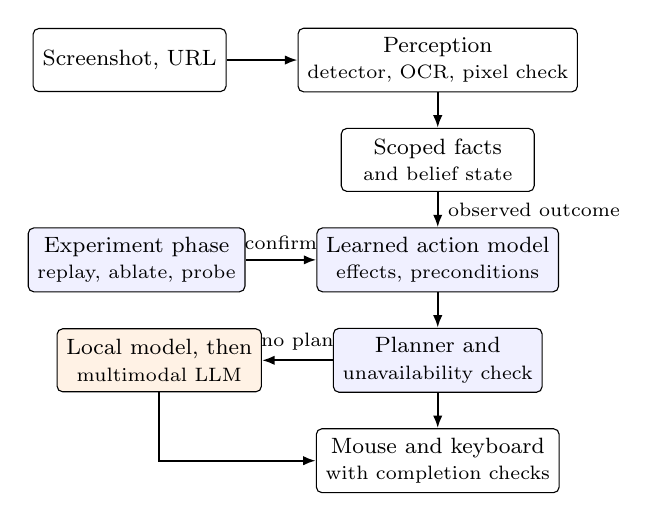
\begin{tikzpicture}[
  box/.style={draw, rounded corners=2pt, align=center, font=\footnotesize, minimum width=2.45cm, minimum height=0.8cm, fill=white},
  learn/.style={box, fill=blue!6},
  llm/.style={box, fill=orange!10},
  arr/.style={-{Latex[length=1.6mm]}, thick},
  lbl/.style={font=\scriptsize, midway}]
\node[box] (screen) {Screenshot, URL};
\node[box, right=0.9cm of screen] (perc) {Perception\\{\scriptsize detector, OCR, pixel check}};
\node[box, below=0.45cm of perc] (facts) {Scoped facts\\{\scriptsize and belief state}};
\node[learn, below=0.45cm of facts] (model) {Learned action model\\{\scriptsize effects, preconditions}};
\node[learn, left=0.9cm of model] (exp) {Experiment phase\\{\scriptsize replay, ablate, probe}};
\node[learn, below=0.45cm of model] (plan) {Planner and\\{\scriptsize unavailability check}};
\node[llm, left=0.9cm of plan] (llm) {Local model, then\\{\scriptsize multimodal LLM}};
\node[box, below=0.45cm of plan] (exec) {Mouse and keyboard\\{\scriptsize with completion checks}};
\draw[arr] (screen) -- (perc);
\draw[arr] (perc) -- (facts);
\draw[arr] (facts) -- node[lbl, right] {observed outcome} (model);
\draw[arr] (exp) -- node[lbl, above] {confirm} (model);
\draw[arr] (model) -- (plan);
\draw[arr] (plan) -- node[lbl, above] {no plan} (llm);
\draw[arr] (plan) -- (exec);
\draw[arr] (llm) |- (exec);
\end{tikzpicture}
\caption{Agent overview. Blue components make no LLM calls. The policy LLM is consulted only when the learned model has no plan; the goal compiler runs once per task.}
\label{fig:architecture}
\end{figure}

\subsection{Perception}
A screen parser detects interactable regions~\cite{lu2024omniparser} and an OCR engine~\cite{du2020ppocr} reads their labels and the surrounding text. Whether a control is enabled is decided from the pixels. The agent compares luminance percentiles of the label's text and background and treats a control as disabled when the ratio is below 3, a level taken from the accessibility guideline for user-interface components~\cite{wcag21} (which itself exempts inactive controls). On labelled screenshots this check never marked an enabled control as disabled (precision 1.00 on every set). It found all 37 disabled controls among 367 controls of the benchmark applications, 102 of 114 among 240 controls styled with four CSS frameworks, and 4 of 14 among 353 controls of a self-hosted real application. On that application it also left 134 labels unread, and all 10 misses were the same control on 10 pages. When the LLM chooses a target whose identity is uncertain, the agent re-grounds it with a second LLM call on a crop that outlines the proposed box (\emph{refinement}). Refinement is skipped for a click on the only enabled control with the cited label, and for a target chosen by the learned model. When no detected element covers the intended target, the LLM can request a \emph{discovery} call that searches the screenshot for it.

\subsection{Facts and belief state}
Status lines longer than about 60 characters, timestamps, and text or controls that appear in every section (the application title, section links) are treated as page chrome and excluded. A persistent inventory records which facts and controls each scope has ever shown. The belief state of a run labels each fact as observed, observed absent (the inventory knows it for the current scope but it is not on screen), predicted (by a learned effect), stale (last seen in another section) or unknown. Unknown facts neither support nor contradict anything. An absence must hold on two consecutive observations before the agent uses it to declare a goal unavailable, so a single OCR miss cannot end a run.

\subsection{Learning from interaction}
After each click the agent compares the facts before and after. A click is \emph{effective} if one of the action's confident effects occurred, \emph{provisional} if facts changed but the action has no confident effect yet, and \emph{ineffective} or \emph{no change} otherwise. For an effective or provisional click, every changed fact adds support to an effect. A fact that appears gives an effect directly; a fact that disappears is credited once some action's appearance of that fact is confident, so that a window closing is learned without crediting every incidental disappearance. After an effective click, every fact that held before it, except the action's own availability, adds support to a candidate precondition, and a candidate that was false although the click worked is contradicted. An ineffective click earns causal credit only inside an experiment, where exactly one fact was withheld (Section~\ref{sec:experiments}). A status fact that no action has ever changed, such as a role line, is a \emph{context condition}. An effect that appears only in another section is credited when the agent returns there, but only if exactly one action happened in between. An effect is confident at support $\ge 2$ and confidence $\ge 0.6$.

\subsection{Experiment phase}
\label{sec:experiments}
Passive learning makes every co-occurring fact a candidate precondition. In \modeActive{} mode, after an application's exploration tasks, the agent runs an experiment phase with its own step budget and no goal, no policy and no LLM call. It resets the application to recorded start states and runs three kinds of experiment (Algorithm~\ref{alg:experiments}):
\begin{enumerate}
\item \emph{Reference replays.} Each exploration run is replayed from its recorded start state. After each replayed click the page is reloaded, and only changes that survive the reload count. A replayed click with a lasting change is a reference: its changes become success effects, and its preconditions gain support.
\item \emph{Tours.} After a reference click, the agent visits sections that show a control believed unavailable, so that a change there is credited to that single action.
\item \emph{Ablated replays.} Each recorded run is replayed with one step left out, which removes the facts that step produced. Every later action is then clicked directly, even if it looks disabled. An action works only if one of its success effects appears. If it still works, each removed fact is refuted as its precondition. If it fails, or its control is missing, while nothing else has diverged, the removed facts are confirmed as one group, since facts that always appear together cannot be told apart.
\end{enumerate}
A precondition becomes \emph{required} after at least two supporting observations, at least one of them an intervention, and no contradiction. One failed ablation plus one passive observation therefore suffices.

\begin{algorithm}[t]
\caption{Experiment phase (no LLM calls)}
\label{alg:experiments}
\begin{algorithmic}[1]
\Require recorded exploration runs $\mathcal{R}$, learned model $M$, step budget $B$
\For{each run $r \in \mathcal{R}$} \Comment{reference replays}
  \State reset the application to the start state of $r$
  \For{each click $a$ in $r$}
    \State replay $a$; reload; $\Delta \gets$ facts changed and kept after reload
    \If{$\Delta \neq \emptyset$} add $\Delta$ to the success effects of $a$; support its preconditions in $M$; tour sections with unavailable controls \EndIf
  \EndFor
\EndFor
\For{each run $r \in \mathcal{R}$ and each step $x$ of $r$} \Comment{ablations}
  \State replay $r$ without $x$; $F_x \gets$ facts produced by $x$
  \For{each later action $a$ of $r$, clicked directly}
    \If{a success effect of $a$ appears} refute each $f \in F_x$ as a precondition of $a$
    \ElsIf{no other fact diverged} confirm $F_x$ as one precondition group of $a$
    \EndIf
  \EndFor
  \State \textbf{stop} when $B$ steps are used
\EndFor
\end{algorithmic}
\end{algorithm}

\subsection{Using the model}
\textbf{Planning.} A goal is split into parts at ``and'', ``then'', commas and semicolons, and each part is matched to the learned effect it asks for. Only effects that make something appear are goal targets. A backward-chaining planner (depth 4, confidence $\ge 0.6$) then chains schemas. It uses an action as is if its control is believed available, makes a disabled or hidden control available through learned availability effects, and establishes required preconditions. It never establishes an unconfirmed candidate: planning through every co-occurring fact would add side-effect steps. When the next schema belongs to another section, the agent clicks the learned link to that section. Learned steps make no LLM calls. In \modePassive{} mode, which has no required preconditions, the planner can therefore only use availability effects, and a precondition that does not show as a disabled control is left to the LLM.

\textbf{Unavailability.} When the planner finds no plan, the agent declares the goal unavailable if a goal part matches the effect of a schema whose context condition (support $\ge 2$) is observed absent on two consecutive observations.

\textbf{Completion checks.} LLM policies often stop after the first part of a multi-part goal. Every goal part that the goal compiler leaves uncovered becomes a constraint in the ledger, and \emph{done} is refused until every part is proven or declared unavailable. A part is proven by a click on a control whose label contains the part's verb, matched on the first five characters, with ``generate'', ``new'', ``add'' and ``make'' accepted for ``create''. The click must also pass its check or produce new status text on the same page. The last open part may instead be proven by the done's own evidence, if that evidence appeared with the latest action that changed the screen. Status text produced by a click that belongs to a proven part stays with that part, so it cannot prove another.

\subsection{Policy, memory and cost}
When the learned model has no plan, a small non-autoregressive local decision model proposes the next action. The multimodal LLM~\cite{gemini2023} decides when the local model abstains, repeats itself or follows a failed step. The LLM runs at its default sampling temperature and receives a set-of-mark screenshot~\cite{yang2023som}, the element list and the constraint ledger. The goal compiler runs at temperature~0. The agent also keeps a graph of screens and transitions. The actions previously taken from the current screen, and whether they worked, are included in the LLM prompt as context. \modeNone{} starts this graph empty in every run, while the two learning modes keep it across runs. In the evaluation this graph never replayed an action by itself. Every LLM call is counted by purpose: policy, refinement, goal compilation and discovery.

% =====================================================================
\section{Benchmark and Protocol}
% =====================================================================
\textbf{Applications.} The benchmark contains three web applications served locally: a project workspace (A: 15 actions in 5 sections), a help desk (B: 11 actions in 4 sections) and an order system (C: 12 actions in 3 sections). Each application has two hidden, two error-style and 7--11 disabled-style controls; controls that depend on the user's role or on earlier actions; and effects that appear in other sections. Each renders in three layouts: classic, compact and reordered.

\textbf{Task groups.} Per agent there are 47 tasks:
\begin{itemize}
\item 8 exploration tasks that together cover every action of A and B;
\item 8 held-out goals and 6 compositions of explored actions;
\item 8 layout-shift tasks that repeat four held-out and composition goals in the two unseen layouts;
\item 9 unavailable tasks, one per application and style, where the control is hidden, disabled or shows an error for the user's role;
\item 8 tasks on application C, which has no exploration phase, run in a fixed order.
\end{itemize}
Each task's step budget is twice its scripted path length plus four.

\textbf{Scoring.} A hidden evaluator records application state that the agent cannot see. An achievable task passes when the final values of the scripted path hold and no other state changed; keys that only record which view is open are ignored. An unavailable task passes when the agent declares it unavailable and changes nothing outside its setup. Learned rules are scored against a ground truth obtained by rendering every reachable state and parsing it with the same perception, so the agent is not penalised for facts it cannot see. A learned precondition is correct if it belongs to the minimal set of facts equivalent to the action's requirements, or to the facts that literally track one requirement. Recall is computed over the actions the agent learned. As a reference, a copy baseline takes every fact true in any reachable state where the action works.

\textbf{Agents and protocol.} We compare three memory modes of the same agent: \modeNone{} (no memory), \modePassive{} (learning from its own tasks) and \modeActive{} (\modePassive{} plus the experiment phase, with a budget of 150 steps). Memory is kept per application, so every application starts with empty memory. For A and then B, each mode runs the exploration tasks, then the experiment phase (\modeActive{} only), then the remaining groups. On C it runs C1--C8 in order and then C's unavailable tasks. The \modePassive{} and \modeActive{} modes run identical code before an application's experiment phase and on C, so their difference on exploration and on C measures run-to-run variation. The LLM is pinned to \texttt{gemini-3.5-flash-lite}. Each mode runs three seeds, with one run per task, mode and seed. Seeds differ in the order of the exploration tasks (one order for seeds 1 and 3, the reverse for seed 2), so that results do not hinge on one exploration order, and the LLM is sampled independently in every run. We report success over the 141 task runs per mode with Wilson 95\% intervals~\cite{wilson1927}, exact McNemar tests on paired task runs, exact sign-flip tests with tasks or goals as units, and mean LLM calls per task. Runs cut short by quota, network or service errors were re-run with the learned memory restored to its state before the run. % RESULT

\textbf{Ablations.} Two variants address the confounds of Section~\ref{sec:discussion}. \modePassive{} \emph{without transition context} removes all previously taken actions and the path from the LLM prompt, including those of the current run that \modeNone{} still sees, and is otherwise unchanged. \modeActive{} \emph{with replay only} runs the reference replays and tours of the experiment phase, under the same 150-step cap, but no ablated replays. Both ran on B with seed 1. Each re-ran B's whole sequence, including its exploration tasks, so its exploration can differ from that of the main mode by run-to-run variation.

% =====================================================================
\section{Results}
\label{sec:results}
% =====================================================================
% RESULT: Table I values (summary.json, "table"; per-seed row from analysis/paper_numbers.py).
\begin{table*}[t]
\centering
\caption{Success (solved/total task runs over three seeds, with Wilson 95\% interval) and mean LLM calls per task, by task group and memory mode. The last row gives the tasks solved out of 47 in seeds 1, 2 and 3.}
\label{tab:main}
\begin{tabular}{l rlr rlr rlr}
\toprule
& \multicolumn{3}{c}{\modeNone} & \multicolumn{3}{c}{\modePassive} & \multicolumn{3}{c}{\modeActive} \\
\cmidrule(lr){2-4}\cmidrule(lr){5-7}\cmidrule(lr){8-10}
Group & solved & 95\% CI & calls & solved & 95\% CI & calls & solved & 95\% CI & calls \\
\midrule
Exploration         & 11/24 & [28, 65] & 18.2 & 10/24 & [24, 61] & 16.0 & 12/24 & [31, 69] & 16.0 \\
Held-out (RQ2)      & 11/24 & [28, 65] & 11.8 & 13/24 & [35, 72] &  6.7 & 16/24 & [47, 82] &  6.1 \\
Composition (RQ3)   & 2/18  & [3, 33]  & 26.2 & 4/18  & [9, 45]  & 14.9 & 10/18 & [34, 75] & 14.2 \\
Layout shift (RQ4)  & 9/24  & [21, 57] & 19.6 & 10/24 & [24, 61] & 15.6 & 20/24 & [64, 93] &  4.4 \\
Unavailable (RQ5)   & 0/27  & [0, 12]  & 10.7 & 9/27  & [19, 52] &  8.3 & 9/27  & [19, 52] &  8.4 \\
No exploration, C (RQ6) & 5/24 & [9, 40] & 16.7 & 8/24 & [18, 53] & 13.9 & 7/24 & [15, 49] & 16.4 \\
\midrule
All                 & 38/141 & [20, 35] & 16.7 & 54/141 & [31, 47] & 12.4 & 74/141 & [44, 61] & 10.7 \\
Per seed (of 47)    & \multicolumn{3}{c}{10, 13, 15} & \multicolumn{3}{c}{18, 17, 19} & \multicolumn{3}{c}{26, 22, 26} \\
\bottomrule
\end{tabular}
\end{table*}

% RESULT: Figure values (same source as Table I). Error bars: += upper, -= lower.
\begin{figure}[t]
\centering
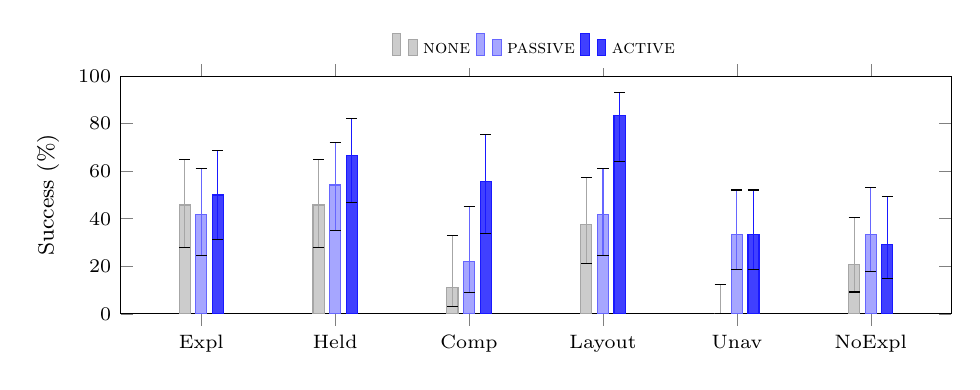
\begin{tikzpicture}
\begin{axis}[
  ybar, width=\columnwidth, height=4.6cm, bar width=4pt,
  ymin=0, ymax=100, ylabel={Success (\%)}, ylabel style={font=\footnotesize},
  symbolic x coords={Expl,Held,Comp,Layout,Unav,NoExpl},
  xtick=data, xticklabel style={font=\scriptsize},
  yticklabel style={font=\scriptsize},
  legend style={font=\scriptsize, at={(0.5,1.03)}, anchor=south, legend columns=3, draw=none},
  error bars/y dir=both, error bars/y explicit,
  error bars/error bar style={line width=0.4pt},
  enlarge x limits=0.12]
\addplot[fill=gray!40, draw=gray!70] coordinates {
  (Expl,45.8) += (0,19.1) -= (0,17.9) (Held,45.8) += (0,19.1) -= (0,17.9) (Comp,11.1) += (0,21.7) -= (0,8.0)
  (Layout,37.5) += (0,19.8) -= (0,16.3) (Unav,0) += (0,12.5) -= (0,0) (NoExpl,20.8) += (0,19.6) -= (0,11.6)};
\addplot[fill=blue!35, draw=blue!60] coordinates {
  (Expl,41.7) += (0,19.5) -= (0,17.2) (Held,54.2) += (0,17.9) -= (0,19.1) (Comp,22.2) += (0,23.0) -= (0,13.2)
  (Layout,41.7) += (0,19.5) -= (0,17.2) (Unav,33.3) += (0,18.8) -= (0,14.7) (NoExpl,33.3) += (0,20.0) -= (0,15.4)};
\addplot[fill=blue!75, draw=blue!90] coordinates {
  (Expl,50.0) += (0,18.6) -= (0,18.6) (Held,66.7) += (0,15.4) -= (0,20.0) (Comp,55.6) += (0,19.9) -= (0,21.8)
  (Layout,83.3) += (0,10.0) -= (0,19.2) (Unav,33.3) += (0,18.8) -= (0,14.7) (NoExpl,29.2) += (0,20.0) -= (0,14.3)};
\legend{\modeNone, \modePassive, \modeActive}
\end{axis}
\end{tikzpicture}
\caption{Success by task group over three seeds, with Wilson 95\% intervals. Groups abbreviate the rows of Table~\ref{tab:main}.}
\label{fig:success}
\end{figure}

\textbf{Overall.} % RESULT
Table~\ref{tab:main} and Fig.~\ref{fig:success} summarise the results. Over three seeds, \modeActive{} solved 74 of 141 task runs (52\%), \modePassive{} 54 (38\%) and \modeNone{} 38 (27\%), and the order was the same in every seed. On the 141 paired task runs, \modeActive{} solved 41 that \modeNone{} failed and lost 5 (exact McNemar $p<0.001$), and \modePassive{} gained 23 and lost 7 ($p=0.005$). \modeActive{} beat \modePassive{} on 26 runs and lost 6 ($p<0.001$). These tests treat the three seeds and three layouts of a goal as independent. Counting each of the 47 tasks once (the number of seeds it was solved in, exact sign-flip test), the differences remain for \modeActive{} against \modeNone{} ($p<0.001$) and \modePassive{} ($p=0.008$), and for \modePassive{} against \modeNone{} ($p=0.04$); grouping the layout variants of each goal, \modeActive{} against \modePassive{} gives $p=0.06$. The two modes run identical code on the exploration tasks and on C, and there they differed on only 9 runs, 5 to 4, which measures run-to-run variation. Where the code differs, after the experiment phase, \modeActive{} won 18 runs and lost none on B, and won 3 and lost 2 on A. Outside B, the two modes solved the same number of runs (27 of 87). Two goals on B, ``escalate ticket \#4821 and save a reply macro'' and ``resolve and close ticket \#4821'', account for 14 of the net 20 runs \modeActive{} won over \modePassive{}. Differences of a few runs within one group are within the run-to-run variation.

\textbf{RQ1: learning from pixels.} % RESULT
Table~\ref{tab:rules} compares the learned rules with the ground truth. Effects are learned accurately: in every seed, confident effects have a precision of 0.93--1.00, with mean recall between 0.31 and 0.76. Passive precondition candidates are imprecise (mean 0.23--0.32), because every fact that happened to be on screen becomes a candidate. The copy baseline has a precision of only 0.05--0.06. Experiments raise precondition precision, on few rules. On B, 9 of 14, 9 of 14 and 9 of 13 preconditions confirmed by experiment are correct in the three seeds (mean precision 0.66), with recall 0.80 in every seed. On A the gain is small and not consistent: 5 of 7, 1 of 3 and 6 of 13 are correct (mean 0.50, against 0.32 for passive candidates; in seed 2, 0.33 against 0.35), with recall 0.14--0.40. The experiment phase also raised effect and candidate recall, since its reference replays add observations without any intervention. On B it ran all 15--19 planned ablated replays within 81--111 steps. On A it used its whole 150-step budget after 8--13 of 16--23, which likely contributes to the lower recall there. For comparison, the exploration tasks themselves took 67--82 steps on A. Context conditions such as role lines were rarely correct (precision 0.00--0.17 per seed). No experiment made an LLM call.

% RESULT: Table II values (summary.json, "rules"; mean over seeds 1-3).
\begin{table}[t]
\centering
\caption{Precision (P) and recall (R) of learned rules against the perception-derived ground truth, over the actions each mode learned, as the mean over three seeds. Models are scored after exploration and, in \modeActive{}, the experiment phase. Effects count as confident at confidence $\ge 0.5$ in this scoring.}
\label{tab:rules}
\footnotesize
\setlength{\tabcolsep}{3.2pt}
\begin{tabular}{l cc cc cc cc}
\toprule
& \multicolumn{4}{c}{App A (workspace)} & \multicolumn{4}{c}{App B (help desk)} \\
\cmidrule(lr){2-5}\cmidrule(lr){6-9}
& \multicolumn{2}{c}{\modePassive} & \multicolumn{2}{c}{\modeActive} & \multicolumn{2}{c}{\modePassive} & \multicolumn{2}{c}{\modeActive} \\
Rule type & P & R & P & R & P & R & P & R \\
\midrule
Effects (confident)       & .95 & .52 & .97 & .69 & 1.00 & .31 & 1.00 & .76 \\
Precond.\ (candidate)     & .32 & .59 & .26 & .86 & .23 & .40 & .25 & .90 \\
Precond.\ (confirmed)     & --  & --  & .50 & .30 & --  & --  & .66 & .80 \\
Context condition         & .00 & .00 & .00 & .00 & .13 & .17 & .12 & .20 \\
\midrule
Copy baseline (P)         & \multicolumn{4}{c}{.05} & \multicolumn{4}{c}{.06} \\
\bottomrule
\end{tabular}
\end{table}

\textbf{RQ2: new goals.} % RESULT
On held-out goals, \modeActive{} solved 16 of 24 runs and \modePassive{} 13, against 11 for \modeNone{}, with 6.1 and 6.7 calls per task against 11.8. Several held-out tasks ran entirely on learned steps. In every seed, both learning modes completed ``assign ticket \#4821 and reply to the customer'' in three learned steps with two LLM calls, where \modeNone{} needed five. In seeds 1 and 3 they also completed ``sign in and share the launch brief'' in five learned steps with three calls; \modeNone{} failed it in every seed. Table~\ref{tab:cost} breaks the cost down over all tasks. The saving comes from fewer policy and refinement calls; the goal compiler costs one call per task in every mode. Part of the saving follows from success itself, because failed runs use up their step budget. On the 33 task runs both \modeActive{} and \modeNone{} solved, \modeActive{} used 4.9 calls against 8.7. On the 62 both failed, it used 18.5 against 20.6. Without application B, the averages are 14.0 for \modeActive{}, 13.8 for \modePassive{} and 17.9 for \modeNone{}.

% RESULT: Table III values computed from the per-run rows (gemini_calls, origins, steps).
\begin{table}[t]
\centering
\caption{Mean LLM calls per task by purpose, steps per task, and share of steps decided by the learned model, over all 141 task runs (three seeds).}
\label{tab:cost}
\begin{tabular}{l rrr}
\toprule
& \modeNone & \modePassive & \modeActive \\
\midrule
Policy                     & 13.1 & 9.8 & 8.3 \\
Refinement                 & 2.0  & 1.2 & 1.1 \\
Goal compilation           & 1.0  & 1.0 & 1.0 \\
Discovery                  & 0.5  & 0.3 & 0.4 \\
Other                      & 0.01 & 0   & 0   \\
\midrule
Total LLM calls            & 16.7 & 12.4 & 10.7 \\
Steps                      & 12.7 & 10.8 & 10.0 \\
Steps by learned model     & 0\%  & 17\% & 23\% \\
\bottomrule
\end{tabular}
\end{table}

\textbf{RQ3: composition.} % RESULT
\modeNone{} solved 2 of 18 composition runs, against 4 for \modePassive{} and 10 for \modeActive{}. The plans combined actions learned in different exploration tasks. In every seed, \modeActive{} completed ``escalate ticket \#4821 and save a reply macro'' with six learned steps and a single LLM call, the goal compiler, and did the same in both unseen layouts. \modePassive{} and \modeNone{} failed this task in all nine runs. In the \modeActive{} model of every seed, ``Priority: urgent'' became a required precondition of escalating the ticket. The phase ended with 6 supporting observations, 2 of them interventions; the final model has 10. In the \modePassive{} model the same fact remained an unconfirmed candidate, which the planner does not establish. This difference follows from the experiments together with the planner's choice to plan only through confirmed preconditions; a passive planner that also planned through frequent candidates might close part of this gap.

\textbf{RQ4: layout shift.} % RESULT
Control identity is the normalised label, not the position, so learned actions transfer to the unseen compact and reordered layouts. \modeActive{} solved 20 of 24 layout-shift runs with 4.4 calls, against 10 for \modePassive{} with 15.6 calls and 9 for \modeNone{} with 19.6. The export workflow, for example, ran in five learned steps with two to four calls in both learning modes, in every layout and seed. For \modeActive{}, every shifted-layout run had the same outcome as the classic-layout run of the same goal and seed, so the gap to \modePassive{} repeats the held-out and composition gaps rather than adding independent evidence.

\textbf{RQ5: knowing when something cannot be done.} % RESULT
No mode ever declared an achievable task unavailable. \modeNone{} declared none of its 27 runs on impossible tasks unavailable. Each learning mode declared 9, the three styles (hidden, disabled and error) on application B in every seed, each time from the learned model with one or two LLM calls. These declarations cite permission lines, ``Approver: yes'' and ``Team lead: yes'', which are context conditions. That rule class is imprecise overall (Table~\ref{tab:rules}), so the mechanism worked on B but is fragile. No mode declared an impossible task on A or C. In 20 of the 81 runs on impossible tasks (11 of them by \modeNone{}) the agent ended with \emph{done} instead, sometimes after doing something else, such as exporting a document that it was not allowed to share. The scorer counts these as failures.

\textbf{RQ6: an application without exploration.} % RESULT
On C, memory starts empty and there is no experiment phase, so \modePassive{} and \modeActive{} run the same code (Table~\ref{tab:curve}). Learning made the second and third tasks cheaper. In every seed, both learning modes solved the second task (``create an order, add an item and apply the discount'') with three LLM calls and two learned steps, while \modeNone{} solved it in two of three seeds with 5.3 calls on average. No mode solved C5--C8, which depend on approving and shipping orders, in any seed, and C4 was solved once. The difference between \modePassive{} and \modeActive{} on C (8 and 7 of 24 runs) is run-to-run variation.

% RESULT: Table IV values from summary.json, "learning_curves" (seeds 1-3).
\begin{table}[t]
\centering
\caption{Application C, tasks in their fixed order: runs solved out of three seeds, with mean LLM calls per run in small type.}
\label{tab:curve}
\setlength{\tabcolsep}{2.6pt}
\begin{tabular}{l cccccccc}
\toprule
Task & C1 & C2 & C3 & C4 & C5 & C6 & C7 & C8 \\
\midrule
\modeNone    & 2\,{\scriptsize 10} & 2\,{\scriptsize 5} & 1\,{\scriptsize 7} & 0\,{\scriptsize 14} & 0\,{\scriptsize 24} & 0\,{\scriptsize 32} & 0\,{\scriptsize 15} & 0\,{\scriptsize 26} \\
\modePassive & 1\,{\scriptsize 10} & 3\,{\scriptsize 3} & 3\,{\scriptsize 5} & 1\,{\scriptsize 7} & 0\,{\scriptsize 24} & 0\,{\scriptsize 29} & 0\,{\scriptsize 8} & 0\,{\scriptsize 26} \\
\modeActive  & 2\,{\scriptsize 10} & 3\,{\scriptsize 3} & 2\,{\scriptsize 6} & 0\,{\scriptsize 9} & 0\,{\scriptsize 22} & 0\,{\scriptsize 33} & 0\,{\scriptsize 23} & 0\,{\scriptsize 25} \\
\bottomrule
\end{tabular}
\end{table}

\textbf{Per application.} % RESULT
The gains concentrate on B: \modeActive{} solved 47 of 54 runs on B with 5.4 calls per task, against 27 for \modePassive{} with 10.0 calls and 17 for \modeNone{} with 14.7. On A all modes solved few tasks (16--20 of 54), and on C 5--8 of 33.

% RESULT: Table V values from analysis/paper_numbers.py ("Ablations on B, seed 1") and summary.json "rules".
\begin{table}[t]
\centering
\caption{Ablations on application B, seed 1 (18 tasks): success, mean LLM calls per task, precision (P) and recall (R) of candidate preconditions, precision of confirmed preconditions, and recall of confident effects.}
\label{tab:ablation}
\footnotesize
\setlength{\tabcolsep}{3pt}
\begin{tabular}{l c r cc c c}
\toprule
& & & \multicolumn{2}{c}{Cand.} & Conf. & Eff. \\
\cmidrule(lr){4-5}
Mode & solved & calls & P & R & P & R \\
\midrule
\modeNone                        & 5/18  & 14.6 & -- & -- & -- & -- \\
\modePassive                     & 10/18 & 8.8  & .21 & .40 & -- & .35 \\
\quad without transition context & 9/18  & 9.9  & .27 & .40 & -- & .35 \\
\modeActive                      & 17/18 & 5.1  & .24 & .90 & .64 & .72 \\
\quad with replay only           & 8/18  & 11.7 & .20 & .90 & -- & .82 \\
\bottomrule
\end{tabular}
\end{table}

\textbf{Ablations.} % RESULT
Table~\ref{tab:ablation} shows the ablations on B. Removing the transition context changed little on this slice: \modePassive{} without it solved 9 of 18 tasks against 10 (it won 1 and lost 2, $p=1.0$) and learned the same effects. On this slice, however, even \modePassive{} against \modeNone{} is not significant (6 won, 1 lost, $p=0.13$), so it cannot detect a moderate effect of the context. Removing the ablated replays removed all of \modeActive{}'s lead. With replay only, it solved 8 of 18 against 17 (it won 0 and lost 9, $p=0.004$), no better than \modePassive{} (1 won, 3 lost, $p=0.63$), and used 11.7 calls per task against 5.1. Eight of its nine losses were in the held-out, composition and layout-shift groups (2 of 4, 0 of 3 and 0 of 4 solved, against 4, 2 and 4); the ninth was an exploration task, before the phase. Reference replays alone learned effects as well as the full phase (recall 0.82) and the same candidate recall (0.90), but by construction they confirm no precondition, so, as in \modePassive{}, the planner has no required precondition to establish. The replay-only phase indicates that, with this planner, the gain needs the interventions rather than the replayed observations. Because it used only 21 of its 150 steps, against 95 for the full phase, it does not show what an equally long interaction without interventions, such as further exploration, would yield.

% =====================================================================
\section{Discussion and Limitations}
\label{sec:discussion}
% =====================================================================
\textbf{External validity.} The applications were built for this benchmark. They show state through explicit status and permission lines, and their unavailable functions are always tied to the user's role. Real applications show state less consistently; the low recall of the pixel check on a real application illustrates the gap. We did not compare against memory baselines from related work, such as workflow memory or exploration notes in the prompt~\cite{wang2025awm,zhang2023appagent}. Evaluating on self-hosted real applications, with such baselines, is our next step.

\textbf{Confounds.} % RESULT
The learning modes differ from \modeNone{} in more than the action model. They also see transitions from earlier runs in the LLM prompt, and \modeActive{} uses extra environment steps for its experiments (150 on A and 81--111 on B). Over all seeds, 11 of \modePassive{}'s 23 and 16 of \modeActive{}'s 41 wins over \modeNone{} used no policy LLM call, so the prompt context cannot directly explain them; the ablation without the context (Table~\ref{tab:ablation}) is too small to rule out a moderate effect on the rest. A phase without ablated replays did no better than \modePassive{}, so on B the gain over passive learning needed the interventions, given a planner that uses only confirmed preconditions. That phase used fewer steps, however, so the ablations do not show what an equally long interaction without interventions would yield, and they cover one application and one seed. The experiment phase also needs resettable start states, which a sandbox can provide but a live application may not.

\textbf{Learning is bounded by exploration.} % RESULT
The model contains only outcomes the agent has seen. On A, the LLM-driven exploration never generated a report in any seed (it clicked the button before selecting a region), so no learning mode could plan that goal later, and it selected reviewers only in seed 3. In seed 2 (reverse exploration order), the learning modes never signed in successfully and so failed ``sign in and share the launch brief'', which they solved from learned steps in the other seeds. The experiment phase replays and varies observed interactions; it cannot discover a success that was never observed. Directed exploration of controls that were never clicked would address this, and it is the main lever for A and C.

\textbf{Completion checks are lenient.} The last open goal part can be proven by any new status text from the latest action that changed the screen, so some runs stop early, for example when the LLM cites an error message as evidence. Because tasks are scored by the final application state, such a stop is a failure and never a false pass.

\textbf{Statistics.} % RESULT
The results come from three seeds with a sampling LLM, one run per task, mode and seed. The Wilson intervals and McNemar tests treat the 141 task runs per mode as independent, although each goal appears in three seeds and up to three layouts, and runs within a seed share learned memory. Their $p$-values are therefore optimistic; the per-task and per-goal sign-flip tests in Section~\ref{sec:results} are the conservative ones, although none of the tests models the memory shared within a seed. The ranking of the modes is the same in every seed. Only the difference between \modeActive{} and \modeNone{}, and the results on B, are clearly separated under every test; most per-group differences are not, and the gain of \modeActive{} over \modePassive{} rests on a few goals of one application. Some evaluation processes were restarted after running out of memory, and each interrupted task was re-run with its memory restored.

% =====================================================================
\section{Conclusion}
% =====================================================================
A screenshot-based agent can learn an explicit, plannable model of an unfamiliar application from its own interaction. Effects are learned with high precision. Experiments that replay and ablate the agent's own runs, without any LLM call, raise the precision of preconditions, although on few rules so far. With this model the agent solved more tasks than the same agent without memory or with passive learning only, in each of three seeds, with fewer LLM calls, although the gain over passive learning came from one of the three applications. It executed whole tasks without the policy LLM, reused learned actions in new combinations and new layouts, and declared some impossible tasks unavailable. On one application and seed, a phase without ablated replays did no better than passive learning. Future work will evaluate on real applications against memory baselines, add directed exploration of untried controls, and extend the ablations to all applications and seeds. An anonymised implementation and the benchmark will be released on acceptance.

\bibliographystyle{IEEEtran}
\bibliography{refs}

\end{document}
